\chapter{Implementation}

\section{Macro-Level Modeling}
The macro-level model constitutes the first operational implementation of the railway digital twin
developed in this work. Its primary objective is to generate a simulation-ready representation of the
Belgian railway network while maintaining a level of abstraction that remains computationally
manageable. Unlike the micro-level model presented later in this thesis, which aims to reproduce the
detailed infrastructure of railway stations and track layouts, the macro-level model focuses on the
connectivity between stations and the movement of trains across the network.

At this level of abstraction, railway stations are represented as nodes and railway connections between
stations are represented as edges. Detailed infrastructure components such as switches, signaling
systems, individual tracks, and platform assignments are intentionally omitted. This simplification
significantly reduces the complexity of the generated network while preserving its overall topology and
operational structure.

The implementation of the macro-level model serves several purposes. First, it validates the complete
workflow required to construct a railway digital twin, from raw infrastructure and operational data to
simulation outputs. Second, it provides an initial environment for evaluating trip generation methods
based on real railway operations. Finally, it establishes a baseline model against which the more
detailed micro-level implementation can later be compared.

The implementation was developed in Python and relies on Apache Spark for large-scale data
processing and SUMO for railway simulation. The complete workflow
consists of four main stages: data processing, railway network generation, trip generation, and
simulation execution.

\subsection{Data Processing Pipeline}
The generation of the macro-level railway model begins with the construction of a data processing
pipeline responsible for transforming heterogeneous railway datasets into a format compatible with
SUMO\@. Railway data originates from a unique source but exhibits significant differences in structure,
granularity, and purpose. Consequently, a preprocessing phase is required before any simulation
artefacts can be generated.

Three categories of data are used within the macro-level model:
\begin{itemize}
    \item \textbf{Railway station data:} contains information describing the geographical location and identification of
    Belgian railway stations.
    
    \item \textbf{Railway connectivity data:} provides information regarding the direct railway links connecting stations.
    
    \item \textbf{Railway punctuality data:} operational records describing the observed movements of trains across the 
    railway network.

\end{itemize}

The preprocessing workflow follows a classical Extract-Transform-Load (ETL) approach. During the
extraction phase, raw datasets are loaded into Apache Spark dataframes. Spark was selected because of
its ability to efficiently process large datasets while providing a unified interface for data transformation
operations. Although the macro-level simulation itself does not require distributed execution, the
volume of punctuality records makes Spark particularly suitable for preprocessing tasks.

Once loaded, the datasets undergo a transformation phase during which inconsistencies are corrected
and the data structure is standardized. Particular attention is paid to geographical information.
Infrastructure datasets and operational datasets do not always use identical coordinate
representations, resulting in small discrepancies between station locations and railway line geometries.
Coordinate normalization procedures are therefore applied to ensure consistency between datasets.

A filtering phase is subsequently performed to restrict the simulation to the geographical area and time
period selected by the user. The simulation generator allows a subset of stations to be specified as
input. In addition to these stations, neighboring stations required to preserve network connectivity are
automatically included in the simulation. This approach reduces computational complexity while
ensuring that realistic routes can still be generated.

The output of the preprocessing pipeline consists of a collection of cleaned datasets containing
standardized station information, station-to-station railway connections, and train circulation records.
These datasets constitute the foundation upon which the simulation network is generated.

\begin{figure}[h]
    \centering
    % \includegraphics[width=0.8\textwidth]{figures/implementation/macro-level-data-processing-pipeline.png}
    \caption{Macro-Level Data Processing Pipeline}
    \label{fig:macro-level-data-processing-pipeline}
\end{figure}


\subsection{Railway Network Generation}
Once the preprocessing phase has been completed, the railway network can be generated. The
objective of this stage is to transform the cleaned infrastructure datasets into a graph representation
that can subsequently be converted into a SUMO railway network.

The process begins with the loading of station information. Each station is uniquely identified by its
official identifier and associated with a geographical position. Internally, station information is stored in
dictionary-based structures that provide efficient access during subsequent processing stages. For each
station, the implementation stores its identifier, name, and geographical coordinates.

After station loading, railway links between stations are reconstructed from the station-to-station
dataset. Each railway connection contains the identifier of the departure station, the identifier of the
arrival station, the physical distance separating the two stations, and the geographical shape describing
the railway corridor.

Unlike a purely abstract graph representation, the implementation preserves the geometry of railway
lines whenever this information is available. Railway corridors are therefore represented as polylines
rather than simple straight segments. This decision improves the visual realism of the generated SUMO
network while preserving the simplicity of the macro-level model.

The resulting railway network can be interpreted as a directed graph $G = (V, E)$, where the set of
vertices $V$ corresponds to railway stations and the set of edges $E$ corresponds to direct railway
connections between stations.

Once the graph has been constructed, a series of XML files compatible with SUMO are generated
automatically. These files include the node definitions, edge definitions, stop definitions, train
definitions, and simulation configuration files required to execute the simulation.

The generated node file contains all stations included in the simulation. Each station is represented as a
SUMO node associated with a unique identifier and geographical coordinates. Similarly, the edge file
contains the railway links connecting stations and specifies the geometry and characteristics of each
connection.

The final step consists of converting these files into a SUMO network using the netconvert utility.
This tool automatically transforms the graph representation into a simulation-ready railway network.
The resulting network preserves the geographical distribution of stations and railway corridors while
remaining significantly simpler than the actual Belgian railway infrastructure.

This abstraction offers several advantages. The resulting network is easy to generate, computationally
efficient, and sufficiently realistic for validating trip generation and operational workflows. However, it
also introduces limitations. Since stations are represented by a single node, infrastructure-level
phenomena such as route conflicts, switch occupation, signal interactions, and platform assignment
cannot be reproduced accurately.


\subsection{Trip Generation}
Once the railway network has been generated, train movements must be created in order to execute
the simulation. Rather than relying exclusively on synthetic traffic generation, the proposed
methodology aims to reconstruct train movements from real operational data.

The punctuality dataset contains records describing successive train passages through railway stations.
Each record includes a train identifier, a station identifier, and temporal information such as planned
departure times and observed departure times. Although these records provide valuable operational
information, they do not directly describe complete train journeys.

A reconstruction process is therefore required to transform isolated station observations into coherent
train routes. For each train and operating day, records are first sorted chronologically according to their
planned departure time. The next station visited by the train is then identified using window-based
operations implemented in Apache Spark.

This procedure allows consecutive station pairs to be extracted and transformed into station-to-station
movements. The resulting dataset can be interpreted as a collection of train trajectories describing the
progression of trains through the railway network.

For each reconstructed movement, a simulation departure time must be computed. Since SUMO
internally represents time as the number of seconds elapsed since the beginning of the simulation,
departure times observed in the punctuality dataset are converted into simulation timestamps. This
conversion is performed by calculating the difference between the planned departure time and the
simulation start date selected by the user.

The reconstructed train movements are subsequently aggregated into complete train journeys. Each
journey contains the train identifier, the sequence of visited stations, and the associated departure
times. These journeys are then translated into SUMO route definitions.

The use of real operational data offers several advantages over purely random traffic generation. First,
it preserves realistic traffic density patterns. Second, it reproduces actual station usage frequencies and
train departure distributions. Finally, it provides a more representative basis for evaluating the
behaviour of the digital twin, since the generated traffic reflects real railway operations rather than
artificial assumptions.


\subsection{Simulation}
After the network and train routes have been generated, the simulation scenario can be executed
within SUMO.

The simulation environment is composed of several complementary files. The node and edge files
define the railway network, while additional files specify train definitions, stop locations, and route
information. All these elements are referenced within a SUMO configuration file that serves as the entry
point for the simulation.

During execution, trains move across the generated station-to-station graph according to the timetable
reconstructed during the trip generation phase. Since the macro-level model does not represent
detailed railway infrastructure, train movements are governed primarily by route definitions and travel
times associated with railway connections.

Several outputs are produced during simulation execution. The tripinfo output contains
information regarding completed train journeys, including travel times and delays. The stopinfo
output records stopping events occurring at stations. Finally, summary files provide aggregated
information concerning the evolution of the simulation.

To facilitate the comparison between simulation outputs and historical operational data, a postprocessing module was 
developed. This module parses the XML files generated by SUMO and convertsthem into CSV datasets following a structure 
similar to the original punctuality data.

The post-processing stage reconstructs both scheduled and simulated arrival and departure times for
each train and station. This conversion makes it possible to directly compare simulation results with real
railway observations and therefore evaluate the validity of the generated digital twin.

The complete workflow implemented in the macro-level model can therefore be summarized as follows:
\begin{enumerate}
    \item Infrastructure and operational data are first preprocessed and standardized.
    \item A station-to-station railway network is then generated and converted into a SUMO network.
    \item Historical punctuality records are subsequently transformed into train routes.
    \item These routes are simulated within SUMO.
    \item The resulting outputs are finally converted into datasets suitable for analysis and validation.
\end{enumerate}


\subsection{Limitations}
Although the macro-level model successfully validates the overall digital twin workflow, it remains limited by the level 
of abstraction used. In this model, stations are represented as single nodes and railway corridors as direct connections 
between stations. As a result, detailed infrastructure elements such as platforms, switches, signaling systems, and 
individual tracks are not explicitly represented, which limits the ability to capture local operational constraints and 
some sources of delay.

The model is also constrained by the available data, particularly for reconstructing exact train routes within complex 
railway infrastructures. In addition, the generated network depends on the quality and completeness of the infrastructure 
and operational datasets used. Nevertheless, this macro-level implementation provides an important first step toward a 
complete railway digital twin, as it validates the proposed framework and supports the development of the more detailed 
micro-level model presented in the following section.


\section{Micro-Level Modeling}
The micro-level railway model aims to reproduce the railway infrastructure with a level of detail sufficient to 
represent individual tracks, switches, and station platforms. This model is designed to capture the operational 
constraints and interactions that occur within railway stations and along track segments, providing a more accurate 
representation of train movements and potential sources of delay. 

\subsection{Data Processing Pipeline}
The data processing pipeline follows a multi-stage Extract–Transform–Load (ETL) process. Infrastructure data is first 
collected from the available railway datasets and transformed into a unified format suitable for network reconstruction. 
The raw geographical information contains track geometries represented as sequences of coordinates describing the railway 
centerlines.

After data cleaning and normalization, several infrastructure extraction algorithms are applied. The first stage consists 
of identifying railway switches from the track topology. These switches constitute the connection points between different 
railway tracks and form the basis of the network graph.

The second stage focuses on platform detection. Stations are associated with nearby track segments using a 
proximity-based matching procedure that assigns platforms to the closest available tracks.

Once platforms have been matched, the network is analysed to identify situations where multiple stations are assigned to 
the same track segment. Such conflicts are resolved through a dedicated track segmentation process that increases the 
granularity of the infrastructure representation while preserving the original geometry.

The resulting infrastructure model is then converted into a graph representation that can be used for route generation 
and simulation. Finally, train trips are generated using either synthetic traffic scenarios or operational railway data 
before being integrated into the SUMO simulation environment.

\subsection{Infrastructure Modeling}
\subsubsection{Switch Detection}
The railway infrastructure is first represented as a graph in which track extremities correspond to nodes and track 
sections correspond to edges. For each node, the number of neighbouring track segments is computed.

Nodes connected to exactly two neighbouring segments are considered part of a continuous railway line and are therefore 
not classified as switches. In contrast, nodes connected to three or more neighbouring segments represent branching or 
merging points and are identified as switches. These locations correspond to operational infrastructure elements that 
allow trains to change routes within the network.

The resulting switch and edge datasets forms the foundation of the micro-level network model and is subsequently used for graph 
construction, route generation, and simulation.

\subsubsection{Platform Detection}
The infrastructure dataset provides the geographical position of railway stations as well as the number of platforms 
available at each station and their heights. However, this information is not directly linked to the track segments 
extracted from the railway network. Consequently, a matching procedure was developed to associate each station platform 
with the most relevant track segments.

The proposed approach relies exclusively on spatial proximity. For each station, the Euclidean distance between the 
station location and nearby track segments is computed. The candidate segments are then ranked according to their 
distance to the station centroid.

Let (N) denote the number of platforms associated with a given station. The algorithm selects the (N) closest track 
segments and assigns them to the station. 

\begin{figure}[h]
    \centering
    % 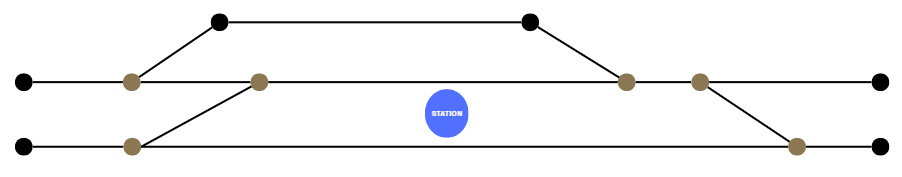
\includegraphics[width=0.6\textwidth]{chapters/images/platform_detection_initial_setup.png}
    \caption{Example of platform detection initial setup}
\end{figure}

For each station, a research zone is defined around its coordinates. 
This research zone is a circular area with an adaptative radius (e.g., 100 meters) that encompasses the area where 
they are likely located. The radius of the research zone can be adjusted based on the density of platforms in the area, 
ensuring that it is large enough to capture all relevant track segments while minimizing the inclusion of irrelevant 
segments.

\begin{figure}[h]
    \centering
    % 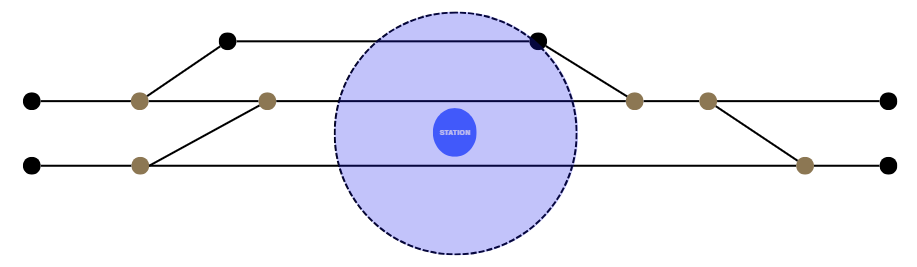
\includegraphics[width=0.6\textwidth]{chapters/images/platform_detection_searching_zone.png}
    \caption{Example of platform detection searching zone}
\end{figure}

This assumption is based on the observation that station platforms are generally located alongside the tracks that serve 
passenger operations. Therefore, the nearest segments constitute a reasonable approximation of the actual platform 
locations while requiring only publicly available infrastructure data.

Within the research zone, the script identifies all track segments from the track dataset that intersect with the zone. 
Then, the script ranks the track segments based on their proximity to the station coordinates. The remaining track 
segments are classified into three categories (given a station that has $n$ platforms):
\begin{enumerate}
    \item Best candidates: the track segments that are closest to the station coordinates and are  likely to correspond to 
    a platform ($rank \le n$).
    \item Mediocre candidates: the track segments that are within the research zone (or close to it) but are not the best 
    candidate. These segments may correspond to additional platforms or other track segments near the station
    ($n \le rank \le 1.5n$).
    \item Irrelevant segments: the track segments that are outside the research zone or are too far from the station 
    coordinates. These segments are unlikely to correspond to platforms and can be disregarded in the platform detection 
    process ($1.5n \le rank \le 2n$).
\end{enumerate}
This ranking approach allows the script to prioritize track segments that are most likely to correspond to platforms 
while minimizing the inclusion of irrelevant segments. By categorizing the track segments based on their proximity to 
the station coordinates, the script can effectively identify potential platform locations and improve the accuracy of 
the platform detection process.

The resulting associations are evaluated using distance-based quality indicators. Stations for which the selected 
segments are located within a short distance are considered to have a high-quality match, whereas larger distances 
indicate potentially less reliable assignments. This quality assessment is later used to analyse the overall accuracy of 
the generated infrastructure model.

\subsubsection{Track Segmentation}
The platform matching process may produce situations in which several stations are associated with the same track segment. 
Such conflicts occur when a single segment represents a long railway section passing through multiple stations, making it 
impossible to uniquely associate each platform with a distinct operational element.

To resolve this issue, an additional track segmentation procedure is applied after the platform matching stage. The 
objective is to increase its operational granularity to ensure that each station platform can be uniquely associated with 
a distinct track segment. 

First, all segments assigned to more than one station are identified. Only these conflicting segments are processed, 
while the remaining network remains unchanged. Each selected segment is then divided into smaller sub-segments according 
to a maximum segment length threshold of 800 meters.

The segmentation process follows the existing geometry of the track. New sub-segments are created exclusively using the 
coordinates already present in the original polyline representation. No interpolation or artificial points are introduced. 
Distances are computed after projecting the geographical coordinates into the Belgian Lambert 72 coordinate system 
(EPSG:31370), allowing accurate metric measurements.

For each generated sub-segment, new extremity nodes are created when necessary and the corresponding track attributes are 
recomputed. The resulting infrastructure therefore preserves the original network geometry while providing a finer 
representation of the railway infrastructure.

After segmentation, the platform matching procedure can be repeated on the newly generated segments. The process 
continues until each station platform is associated with a distinct segment. In practice, a single segmentation iteration 
was sufficient to eliminate all observed conflicts in the Belgian railway network dataset.

This approach allows the model to maintain a realistic infrastructure representation while ensuring that stations and 
platforms can be uniquely mapped to simulation entities. Such a requirement is particularly important for subsequent 
routing, timetable generation, and railway traffic simulation tasks.


\subsubsection{Dual Graph Construction}


\subsection{Trip Generation}
\subsubsection{Random Trips}

\subsubsection{Real Data Trips}


\subsection{Simulation}


\subsection{Limitations}